% !TEX root = ../main.tex
\documentclass[11pt,a4paper]{article}

% ============================================================
% PACKAGES
% ============================================================
\usepackage[indonesian]{babel}
\usepackage{geometry}
\usepackage{graphicx}
\usepackage{setspace}
\setstretch{1.15}
\usepackage{xcolor}
\usepackage{colortbl}
\usepackage{fancyhdr}
\usepackage{titlesec}
\usepackage{tocloft}
\usepackage{float}
\usepackage[justification=centering]{caption}
\usepackage{subcaption}
\usepackage{enumitem}
\setlist{nosep}
\usepackage{amsmath,amssymb}
\usepackage{mathptmx} % Times New Roman typography
\usepackage{tikz}
\usepackage{tcolorbox}
\tcbuselibrary{skins,breakable}
\usepackage[hidelinks,hypertexnames=false]{hyperref}

% ============================================================
% PAGE GEOMETRY & MARGINS
% ============================================================
\geometry{
    top=3cm,
    bottom=3cm,
    left=3.5cm,
    right=2.5cm,
    headheight=16pt,
    headsep=14pt,
    footskip=36pt
}
\emergencystretch=2em

% ============================================================
% BRANDING COLOR PALETTE (Ecological Precision)
% ============================================================
\definecolor{deepgreen}{HTML}{022C22}
\definecolor{mediumgreen}{HTML}{15803D}
\definecolor{lightgreen}{HTML}{DCFCE7}
\definecolor{emeraldgreen}{HTML}{059669}
\definecolor{bordergreen}{HTML}{86EFAC}
\definecolor{darkslate}{HTML}{0F172A}
\definecolor{mutedgray}{HTML}{64748B}
\definecolor{warnamber}{HTML}{D97706}
\definecolor{lightamber}{HTML}{FEF3C7}

% ============================================================
% SECTION & HEADING FORMATTING
% ============================================================
\titleformat{\section}[block]
  {\normalfont\Large\bfseries\color{deepgreen}}
  {\thesection.}
  {0.6em}
  {}
\titlespacing*{\section}{0pt}{18pt plus 4pt minus 2pt}{8pt plus 2pt minus 2pt}

\titleformat{\subsection}[block]
  {\normalfont\large\bfseries\color{mediumgreen}}
  {\thesubsection}
  {0.6em}
  {}
\titlespacing*{\subsection}{0pt}{14pt plus 3pt minus 2pt}{6pt plus 2pt minus 2pt}

\titleformat{\subsubsection}[block]
  {\normalfont\normalsize\bfseries\color{darkslate}}
  {\thesubsubsection}
  {0.5em}
  {}
\titlespacing*{\subsubsection}{0pt}{10pt plus 2pt minus 1pt}{4pt plus 1pt minus 1pt}

% Numbering depth
\setcounter{secnumdepth}{3}
\setcounter{tocdepth}{3}

% ============================================================
% TOC & LOF FORMATTING
% ============================================================
\addto\captionsindonesian{
  \renewcommand{\contentsname}{DAFTAR ISI}
  \renewcommand{\listfigurename}{DAFTAR GAMBAR}
  \renewcommand{\listtablename}{DAFTAR TABEL}
}

\renewcommand{\cfttoctitlefont}{\hfill\Large\bfseries\color{deepgreen}}
\renewcommand{\cftaftertoctitle}{\hfill}
\renewcommand{\cftloftitlefont}{\hfill\Large\bfseries\color{deepgreen}}
\renewcommand{\cftafterloftitle}{\hfill}

\renewcommand{\cftsecleader}{\cftdotfill{\cftdotsep}}
\renewcommand{\cftdotsep}{2}

% Figure numbering
\counterwithin{figure}{section}
\renewcommand{\thefigure}{\arabic{section}.\arabic{figure}}

% ============================================================
% HEADER & FOOTER
% ============================================================
\fancypagestyle{fancy}{
    \fancyhf{}
    \fancyhead[L]{\small\textcolor{mediumgreen}{\textbf{RekaKarbon} -- Buku Panduan Penggunaan Sistem}}
    \fancyhead[R]{\small\textcolor{mutedgray}{\textsf{\manualversion}}}
    \renewcommand{\headrulewidth}{1.2pt}
    \renewcommand{\headrule}{{\color{mediumgreen}\hrule width\headwidth height\headrulewidth}}
    \fancyfoot[L]{\small\textcolor{deepgreen}{\teamname\ | \universityname}}
    \fancyfoot[R]{\colorbox{deepgreen}{\makebox[1.8em][c]{\strut\color{white}\bfseries\thepage}}}
    \renewcommand{\footrulewidth}{0.8pt}
    \renewcommand{\footrule}{{\color{bordergreen}\hrule width\headwidth height\footrulewidth}}
}

\fancypagestyle{plain}{
    \fancyhf{}
    \fancyhead[L]{\small\textcolor{mediumgreen}{\textbf{RekaKarbon} -- Buku Panduan Penggunaan Sistem}}
    \fancyhead[R]{\small\textcolor{mutedgray}{\textsf{\manualversion}}}
    \renewcommand{\headrulewidth}{1.2pt}
    \renewcommand{\headrule}{{\color{mediumgreen}\hrule width\headwidth height\headrulewidth}}
    \fancyfoot[L]{\small\textcolor{deepgreen}{\teamname\ | \universityname}}
    \fancyfoot[R]{\colorbox{deepgreen}{\makebox[1.8em][c]{\strut\color{white}\bfseries\thepage}}}
    \renewcommand{\footrulewidth}{0.8pt}
    \renewcommand{\footrule}{{\color{bordergreen}\hrule width\headwidth height\footrulewidth}}
}

% ============================================================
% CALLOUT / NOTIFICATION BOXES
% ============================================================
\newtcolorbox{infobox}[1][Catatan Penting]{
    enhanced,
    colback=lightgreen!35,
    colframe=mediumgreen,
    arc=4pt,
    boxrule=1pt,
    left=12pt,
    right=12pt,
    top=8pt,
    bottom=8pt,
    title={\textbf{\textcolor{deepgreen}{#1}}},
    coltitle=deepgreen,
    attach boxed title to top left={yshift=-2mm, xshift=4mm},
    boxed title style={colback=lightgreen, boxrule=0.5pt, colframe=mediumgreen, arc=2pt}
}

\newtcolorbox{warningbox}[1][Peringatan]{
    enhanced,
    colback=lightamber!40,
    colframe=warnamber,
    arc=4pt,
    boxrule=1pt,
    left=12pt,
    right=12pt,
    top=8pt,
    bottom=8pt,
    title={\textbf{\textcolor{warnamber}{#1}}},
    coltitle=warnamber,
    attach boxed title to top left={yshift=-2mm, xshift=4mm},
    boxed title style={colback=lightamber, boxrule=0.5pt, colframe=warnamber, arc=2pt}
}

\newtcolorbox{tipbox}[1][Petunjuk Penggunaan]{
    enhanced,
    colback=white,
    colframe=emeraldgreen,
    arc=4pt,
    boxrule=1pt,
    left=12pt,
    right=12pt,
    top=8pt,
    bottom=8pt,
    title={\textbf{\textcolor{emeraldgreen}{#1}}},
    coltitle=emeraldgreen,
    attach boxed title to top left={yshift=-2mm, xshift=4mm},
    boxed title style={colback=white, boxrule=0.5pt, colframe=emeraldgreen, arc=2pt}
}


% ============================================================
% CONFIGURATION / METADATA PANDUAN
% ============================================================
\newcommand{\manualtitle}{REKAKARBON: Platform dMRV Emisi Berbasis AI dan Konsorsium Blockchain Hyperledger Besu}
\newcommand{\manualsubtitle}{Optimalisasi Tata Kelola Emisi Guna Meminimalisir Risiko Greenwashing dan Mewujudkan Indonesia Net Zero}
\newcommand{\manualversion}{v1.0 (KMIPN VIII 2026)}
\newcommand{\teamname}{What Time Is It?}
\newcommand{\universityname}{POLITEKNIK NEGERI MALANG}

\begin{document}

% 1. Halaman Sampul (Cover)
% !TEX root = ../main.tex
\begin{titlepage}
    \thispagestyle{empty}
    \centering

    % Top Category Banner
    \vspace*{0.5cm}
    {\small\textbf{\textcolor{mediumgreen}{\MakeUppercase{Kompetisi Mahasiswa Informatika Politeknik Nasional (KMIPN) VIII 2026}}}}\\[0.2cm]
    {\small\textbf{\textcolor{darkslate}{Kategori: e-Government}}}\\[1.0cm]

    % Document Title
    {\Huge \textbf{\textcolor{deepgreen}{BUKU PANDUAN PENGGUNA}}}\\[0.2cm]
    {\LARGE \textbf{\textcolor{emeraldgreen}{(USER MANUAL BOOK)}}}\\[0.6cm]
    \rule{0.75\textwidth}{1.5pt}\\[0.6cm]
    {\Large \textbf{\textcolor{darkslate}{\manualtitle}}}\\[0.3cm]
    {\normalsize \textit{\textcolor{mutedgray}{\manualsubtitle}}}\\[1.2cm]

    % System & University Logos
    \begin{figure}[H]
        \centering
        \begin{subfigure}[b]{0.35\textwidth}
            \centering
            
\includegraphics[height=3.2cm]{assets/logo-rekakarbon.jpeg}
        \end{subfigure}
        \hspace{1.0cm}
        \begin{subfigure}[b]{0.35\textwidth}
            \centering
            
\includegraphics[height=3.2cm]{assets/logo-polinema.png}
        \end{subfigure}
    \end{figure}

    \vspace{0.8cm}

    % Authors & Metadata
    {\large \textbf{\textcolor{deepgreen}{Disusun Oleh:}}}\\[0.2cm]
    {\normalsize \textbf{\teamname}}\\[0.3cm]
    \begin{tabular}{r c l}
        \textbf{Ekya Muhammad Hasfi Fadlilurrahman} & -- & NIM 2341720111 \\
        \textbf{Farrel Augusta Dinata} & -- & NIM 2341720081 \\
        \textbf{Petrus Tyang Agung Rosario} & -- & NIM 2341720227 \\
    \end{tabular}

    \vfill

    % Institution & Year
    {\large \textbf{\textcolor{deepgreen}{\MakeUppercase{\universityname}}}}\\[0.15cm]
    {\normalsize \textbf{\textcolor{darkslate}{JURUSAN TEKNOLOGI INFORMASI}}}\\[0.15cm]
    {\normalsize \textbf{\textcolor{darkslate}{MALANG}}}\\[0.2cm]
    {\normalsize \textbf{\textcolor{mutedgray}{2026}}}

\end{titlepage}


% 2. Daftar Isi (Table of Contents)
\newpage
\pagenumbering{roman}
\pagestyle{fancy}
\tableofcontents
\addcontentsline{toc}{section}{DAFTAR ISI}

% 3. Daftar Gambar (Table of Images / Figures)
\newpage
\listoffigures
\addcontentsline{toc}{section}{DAFTAR GAMBAR}

% 4. Konten Utama Buku Panduan (Main Manual Book Guideline)
\newpage
\pagenumbering{arabic}
\pagestyle{fancy}
% !TEX root = ../main.tex

% ============================================================
% BAB 1: GAMBARAN UMUM SISTEM REKAKARBON
% ============================================================
\section{Gambaran Umum Sistem RekaKarbon}

\subsection{Tentang Platform RekaKarbon}
\textbf{RekaKarbon} adalah platform \textit{e-government} terintegrasi yang dirancang untuk mendukung siklus \textit{digital Measurement, Reporting, and Verification} (dMRV) emisi karbon nasional secara transparan, akurat, dan terdesentralisasi. Dikembangkan khusus untuk merespons tantangan risiko \textit{greenwashing} dalam perdagangan karbon dan pelaporan emisi industri, RekaKarbon menggabungkan kecerdasan buatan (\textit{Artificial Intelligence}) penginderaan jauh berbasis citra satelit/drone dengan teknologi konsorsium \textit{blockchain} Hyperledger Besu.

Platform ini menjadi jembatan kolaborasi antara regulator pemerintah (KLHK dan Kementerian ESDM), pelaku industri penghasil emisi (\textit{emitters}), kelompok tani hutan pengelola serapan karbon (KTH), serta auditor lingkungan independen.

\begin{figure}[H]
    \centering
    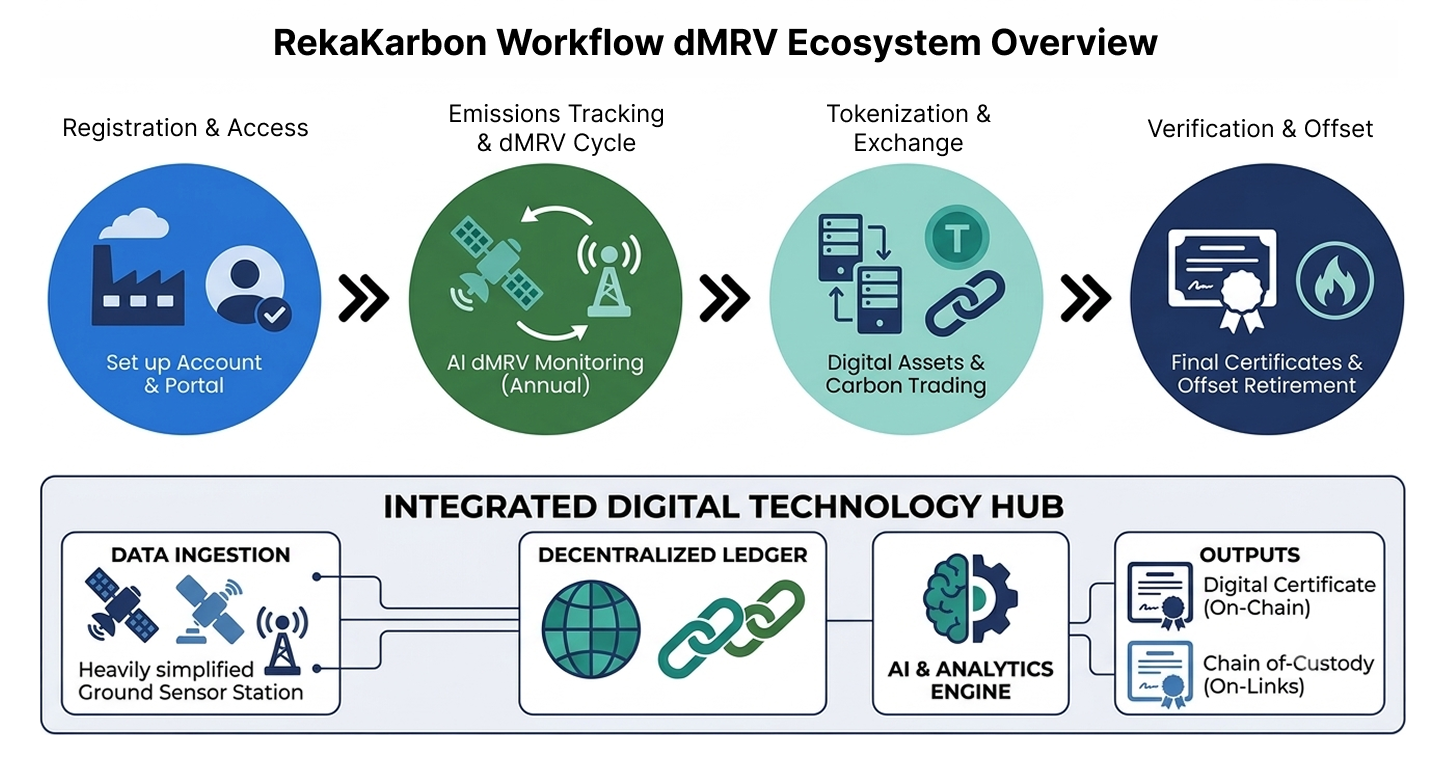
\includegraphics[width=0.92\textwidth]{assets/workflow-dmrv.png}
    \caption{Alur Kerja Ekosistem dMRV Terintegrasi Platform RekaKarbon}
    \label{fig:workflow-dmrv}
\end{figure}

\subsection{Prasyarat Sistem \& Kebutuhan Perangkat Keras}
Untuk dapat menggunakan platform RekaKarbon secara optimal, pengguna disarankan memenuhi spesifikasi teknis berikut:
\begin{enumerate}[label=\alph*.]
    \item \textbf{Peramban Web (Browser)}: Google Chrome (versi 118+), Mozilla Firefox (versi 119+), Microsoft Edge (versi 118+), atau Safari (versi 17+).
    \item \textbf{Koneksi Internet}: Kecepatan pita lebar minimum 5 Mbps untuk kelancaran rendering peta geospasial dan citra satelit resolusi tinggi.
    \item \textbf{Dukungan Web3 / Dompet Digital}: Platform telah dilengkapi arsitektur \textit{sponsored gasless relayer}, sehingga pengguna tidak diwajibkan membeli token bahan bakar jaringan (\textit{native gas}) untuk melakukan transaksi pencatatan sertifikat atau verifikasi data pada \textit{blockchain}.
\end{enumerate}

\begin{tipbox}[Kemudahan Pengguna (Gasless Experience)]
Pengguna tidak perlu memasang dompet ekstensi pihak ketiga (seperti MetaMask) atau memiliki saldo kripto untuk bertransaksi. Seluruh biaya gas transaksi on-chain ditangani secara transparan oleh layanan \textit{Relayer} resmi RekaKarbon.
\end{tipbox}

% ============================================================
% BAB 2: MATRIKS PERAN & HAK AKSES PENGGUNA
% ============================================================
\section{Matriks Peran dan Hak Akses Pengguna}

Sistem RekaKarbon mengimplementasikan sistem kendali akses berbasis peran (\textit{Role-Based Access Control} / RBAC) yang ketat guna memastikan pembagian kewenangan (*segregation of duties*) dan keamanan data emisi nasional:

\begin{table}[H]
\centering
\small
\renewcommand{\arraystretch}{1.25}
\begin{tabular}{|p{3.2cm}|p{5.0cm}|p{5.5cm}|}
\hline
\rowcolor{lightgreen}
\textbf{Peran Pengguna} & \textbf{Deskripsi \& Entitas} & \textbf{Cakupan Fitur Utama} \\
\hline
\textbf{Publik (Tamu)} & Masyarakat umum, akademisi, dan organisasi pemerhati iklim. & Mengakses portal transparansi publik, memeriksa statistik emisi nasional, dan memvalidasi keaslian sertifikat karbon via hash/QR code. \\
\hline
\textbf{Pelaku Usaha (\textit{Emitter})} & Korporasi atau pabrik industri yang menghasilkan emisi GRK. & Pemantauan sensor CEMS, input laporan emisi, pengajuan alokasi PTBAE-PU, kalkulator offset, transaksi di Bursa Karbon, dan retirasi sertifikat. \\
\hline
\textbf{Kelompok Tani Hutan (KTH)} & Komunitas lokal pengelola kawasan konservasi atau reboisasi hutan. & Pendaftaran poligon lahan (GeoJSON), pemantauan biomassa dan stok karbon berbasis AI satelit, serta penerbitan kredit karbon. \\
\hline
\textbf{Auditor Independen} & Lembaga Validasi/Verifikasi (LVV) terakreditasi independen. & Audit laporan emisi CEMS industri, verifikasi data geospasial satelit \& drone, inspeksi IoT gate, dan penerbitan laporan audit digital. \\
\hline
\textbf{Regulator} & Kementerian LHK dan instansi pembina sektor teknis. & Penetapan kuota batas atas emisi (PTBAE-PU), persetujuan penerbitan SPE-GRK, penugasan tim auditor, dan monitoring kepatuhan nasional. \\
\hline
\textbf{Administrator} & Tim pengelola operasional sistem RekaKarbon. & Verifikasi identitas korporasi (\textit{Know Your Business} / KYB), manajemen akun pengguna, audit log sistem, dan kesehatan node jaringan. \\
\hline
\end{tabular}
\caption{Matriks Peran dan Hak Akses Pengguna Sistem RekaKarbon}
\label{tab:role-matrix}
\end{table}

% ============================================================
% BAB 3: PANDUAN PENGOPERASIAN FITUR UTAMA
% ============================================================
\section{Panduan Pengoperasian Fitur Utama}

\subsection{Autentikasi dan Pengaturan Akun}
\begin{enumerate}
    \item Buka peramban dan akses alamat portal resmi RekaKarbon.
    \item Klik tombol \textbf{Masuk} pada pojok kanan atas halaman beranda.
    \item Masukkan alamat email institusi dan kata sandi yang telah didaftarkan.
    \item Apabila akun Anda mewakili korporasi industri baru atau kelompok tani, Anda akan diarahkan ke halaman \textbf{Verifikasi KYB} untuk mengunggah dokumen legalitas (NIB, SK Kemenkumham, atau SK Penetapan Perhutanan Sosial).
\end{enumerate}

\begin{infobox}[Verifikasi Identitas Organisasi (KYB)]
Fitur pelaporan emisi dan transaksi bursa baru akan aktif secara otomatis setelah berkas KYB organisasi diverifikasi dan disetujui oleh Administrator Sistem dalam kurun waktu 1x24 jam kerja.
\end{infobox}

\subsection{Panduan untuk Pelaku Usaha (Emitter)}

\subsubsection{Pemantauan Emisi dan Integrasi CEMS}
\begin{enumerate}
    \item Masuk ke menu \textbf{Laporan Emisi} pada bilah navigasi samping.
    \item Sistem menampilkan metrik waktu nyata konsentrasi gas buang ($SO_2$, $NO_x$, $CO_2$, dan Partikulat) yang tersinkronisasi langsung dari perangkat \textit{Continuous Emission Monitoring System} (CEMS) cerobong pabrik.
    \item Klik \textbf{Unduh Rekapitulasi Periode} untuk mencetak laporan kepatuhan berkala dalam format PDF bersertifikat digital.
\end{enumerate}

\subsubsection{Pengajuan Kuota PTBAE-PU dan Kalkulator Karbon}
\begin{enumerate}
    \item Akses submenu \textbf{Pengajuan PTBAE-PU}.
    \item Masukkan kapasitas produksi historis dan batas intensitas emisi sektor industri Anda.
    \item Gunakan \textbf{Kalkulator Karbon} terintegrasi untuk memperkirakan potensi surplus atau defisit kuota emisi sebelum batas akhir tahun berjalan.
    \item Klik \textbf{Kirim Pengajuan Kuota} untuk diteruskan ke Kementerian LHK.
\end{enumerate}

\subsubsection{Perdagangan di Bursa Karbon DEX dan Retirasi Sertifikat}
\begin{figure}[H]
    \centering
    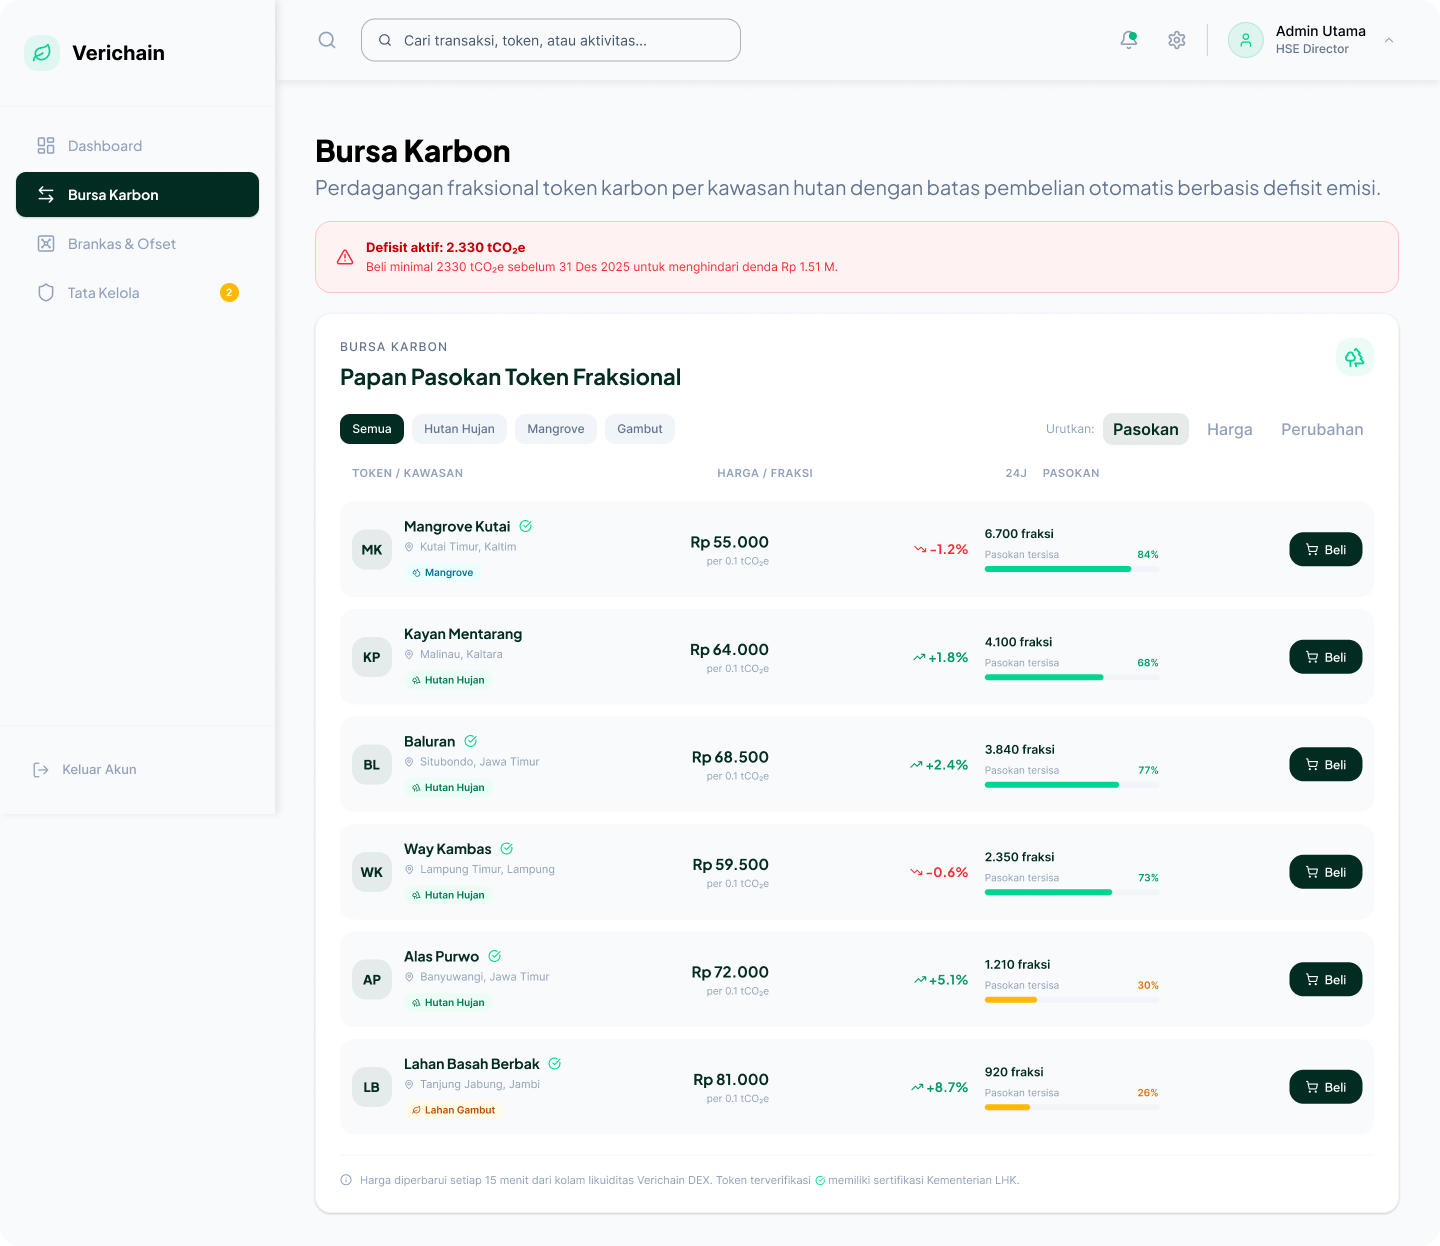
\includegraphics[width=0.88\textwidth]{assets/ui-bursa.png}
    \caption{Antarmuka Bursa Perdagangan Karbon Terdesentralisasi (\textit{Carbon DEX})}
    \label{fig:ui-bursa}
\end{figure}

\begin{enumerate}
    \item Buka menu \textbf{Bursa Karbon}.
    \item Pada tab \textit{Marketplace}, pengguna dapat melihat daftar penawaran Sertifikat Pengurangan Emisi Gas Rumah Kaca (SPE-GRK) yang telah terverifikasi.
    \item Masukkan jumlah volume karbon ($tCO_2e$) yang ingin dibeli atau dioffset, kemudian klik \textbf{Beli Unit Karbon}.
    \item Untuk mengklaim kepatuhan emisi tahunan, buka menu \textbf{Dompet Karbon} $\rightarrow$ pilih sertifikat $\rightarrow$ klik tombol \textbf{Retirasi Sertifikat (Burn)}. Unit karbon tersebut akan dibakar (\textit{burn}) secara permanen di blockchain dan menerbitkan bukti \textit{Certificate of Retirement} yang tidak dapat diperdagangkan kembali.
\end{enumerate}

\subsection{Panduan untuk Kelompok Tani Hutan (KTH)}

\subsubsection{Registrasi Wilayah Hutan dan Unggah Poligon Spasial}
\begin{enumerate}
    \item Masuk ke menu \textbf{Lahan Hutan \& Poligon}.
    \item Klik tombol \textbf{Tambah Wilayah Konservasi Baru}.
    \item Masukkan data administratif kawasan (nama KTH, nomor SK Perhutanan Sosial, jenis tutupan pohon).
    \item Unggah berkas batas wilayah dalam format standard \textbf{GeoJSON} atau \textbf{Shapefile (.shp)}.
    \item Sistem akan secara otomatis memvalidasi koordinat batas lahan agar tidak tumpang tindih (\textit{zero-overlap check}) dengan konsesi lain.
\end{enumerate}

\subsubsection{Monitoring Biomassa AI dan Klaim Kredit Karbon}
\begin{enumerate}
    \item Setelah poligon disetujui, modul AI \textit{NusaCarbon Environmental Intelligence} secara otomatis menganalisis citra satelit Sentinel-2 dan Landsat secara berkala.
    \item Pengguna dapat memantau estimasi \textit{Above Ground Biomass} (AGB) dan serapan karbon bersih bulanan.
    \item Klik \textbf{Ajukan Klaim Kredit Karbon} untuk meminta verifikasi lapangan oleh auditor independen.
\end{enumerate}

\subsection{Panduan untuk Auditor Independen}

\begin{figure}[H]
    \centering
    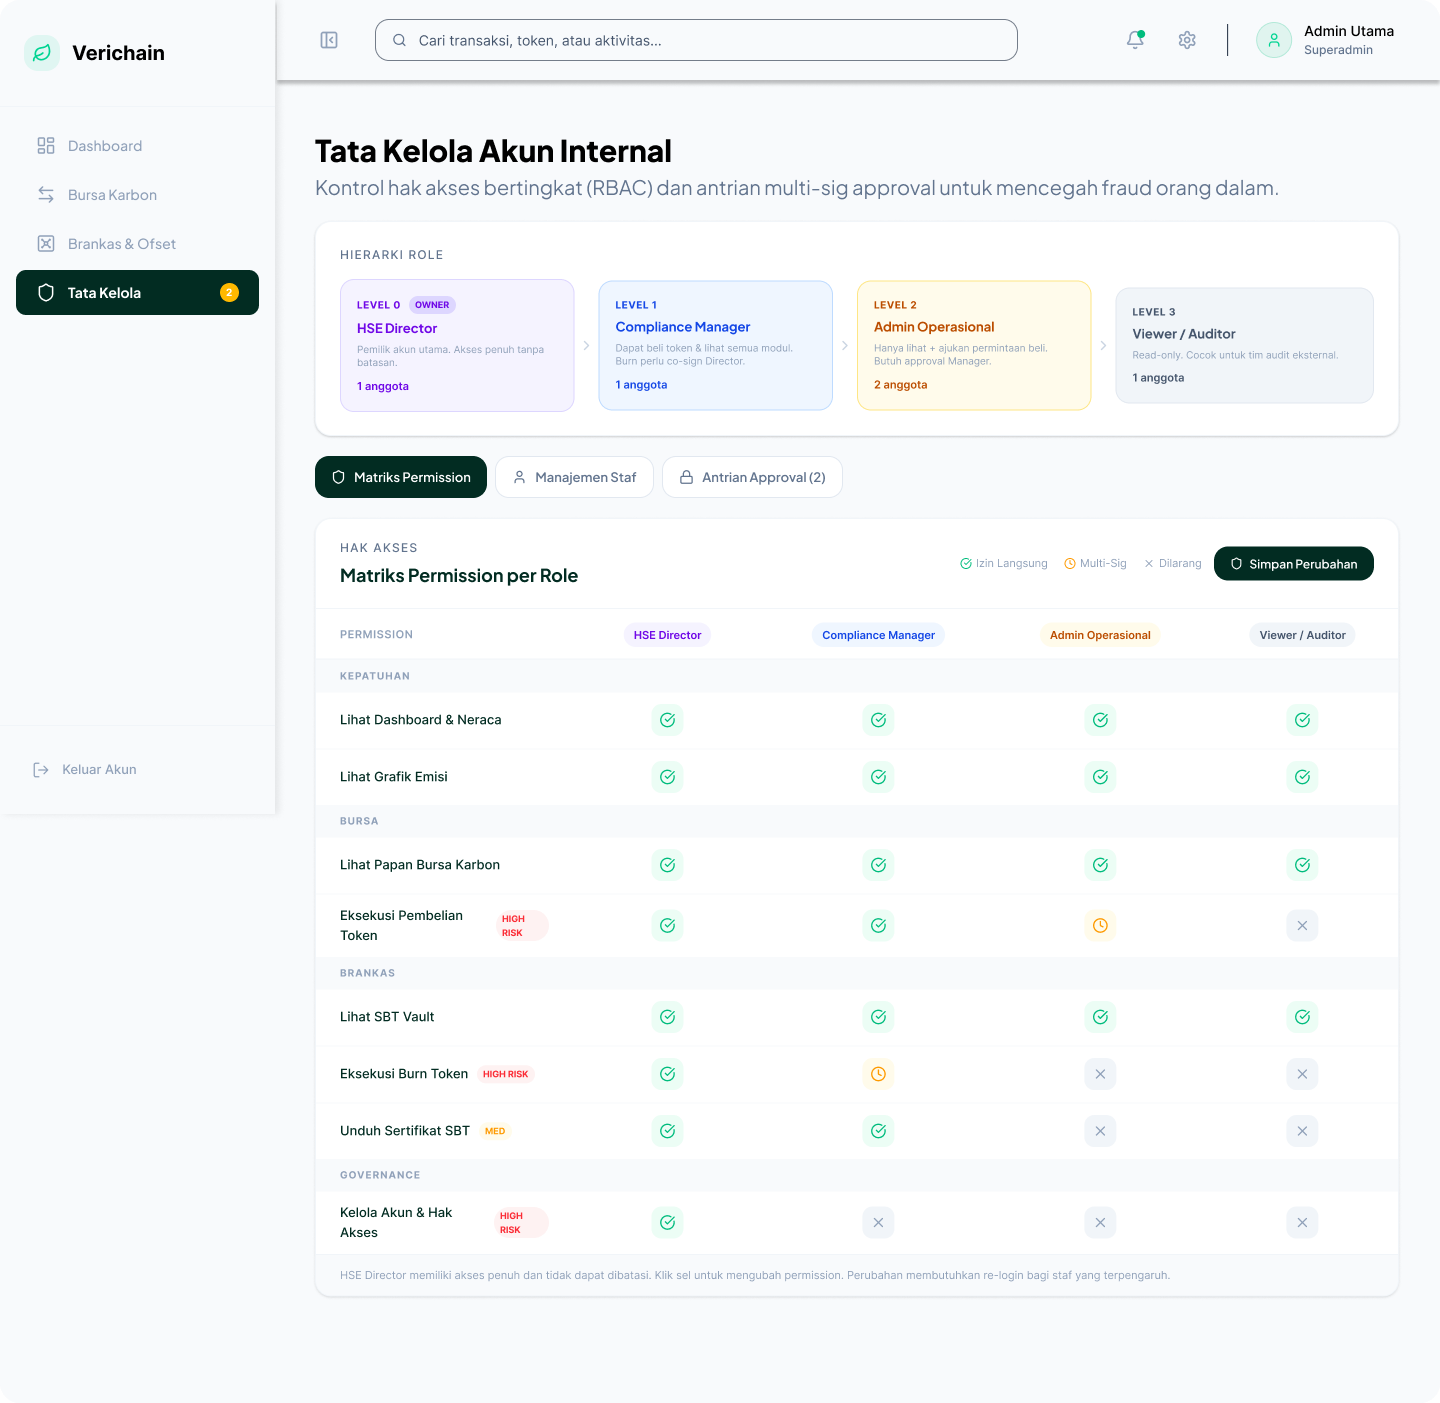
\includegraphics[width=0.88\textwidth]{assets/ui-tata-kelola.png}
    \caption{Dasbor Tata Kelola Audit dan Pemantauan Emisi Digital}
    \label{fig:ui-tata-kelola}
\end{figure}

\subsubsection{Tinjauan Laporan Emisi dan Deteksi Anomali AI}
\begin{enumerate}
    \item Masuk ke menu \textbf{Audit Emisi}.
    \item Buka penugasan audit yang berstatus \textit{Pending Verification}.
    \item Periksa grafik histori data CEMS; sistem secara cerdas akan menandai titik-titik data anomali (\textit{outliers}) yang terdeteksi oleh model machine learning.
    \item Masukkan catatan temuan audit pada kolom \textbf{Lembar Kerja Auditor}.
\end{enumerate}

\subsubsection{Verifikasi Spasial, Drone, dan Gate IoT}
\begin{enumerate}
    \item Buka menu \textbf{Audit Spasial \& Drone}.
    \item Bandingkan data kanopi pohon aktual hasil foto udara drone dengan estimasi biomassa model AI.
    \item Periksa log pencatatan sensor gerbang pengawasan (\textit{IoT Gate}) untuk memastikan tidak ada pembalakan liar di area proyek.
    \item Klik \textbf{Terbitkan Rekomendasi Validasi} untuk menandatangani berita acara audit secara kriptografis menggunakan kunci verifikator.
\end{enumerate}

\subsection{Panduan untuk Regulator (KLHK / ESDM)}
\begin{enumerate}
    \item Masuk ke menu \textbf{Proyek Karbon \& Kuota}.
    \item Evaluasi permohonan sertifikasi SPE-GRK yang telah dilengkapi berita acara verifikasi auditor.
    \item Tinjau alokasi kuota emisi batas atas sektor industri pada menu \textbf{Alokasi PTBAE-PU}.
    \item Klik tombol \textbf{Setujui \& Minting Token} untuk mengesahkan penerbitan unit karbon ke buku besar \textit{blockchain} Hyperledger Besu secara resmi.
\end{enumerate}

\subsection{Panduan Portal Transparansi Publik}
\begin{figure}[H]
    \centering
    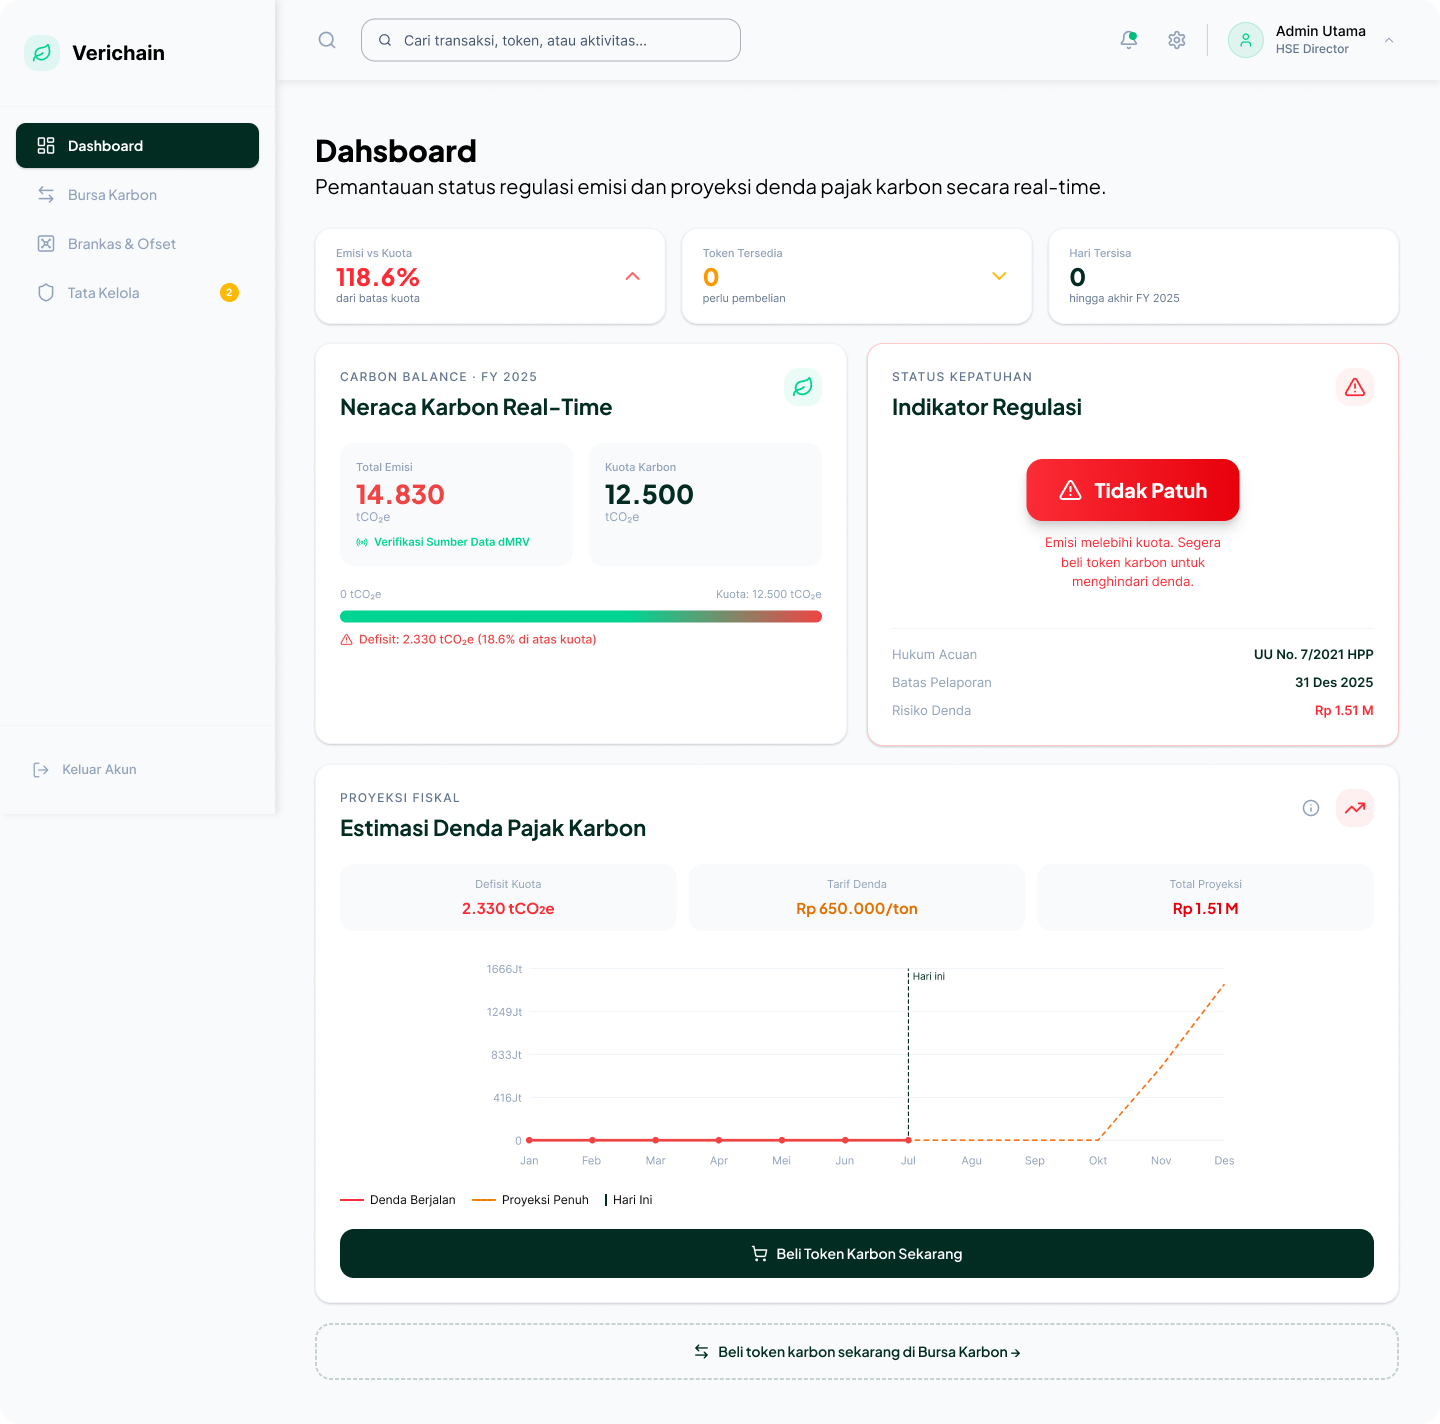
\includegraphics[width=0.88\textwidth]{assets/ui-dashboard.png}
    \caption{Dasbor Transparansi Publik untuk Pengawasan Keterbukaan Data Emisi}
    \label{fig:ui-dashboard}
\end{figure}

Masyarakat umum dapat mengakses portal tanpa perlu melakukan registrasi akun:
\begin{enumerate}
    \item Buka halaman utama dan pilih menu \textbf{Portal Transparansi}.
    \item Pilih sektor industri atau wilayah untuk melihat agregasi emisi karbon yang dilaporkan.
    \item Untuk memverifikasi sertifikat emisi atau kredit karbon fisik:
    \begin{itemize}
        \item Buka submenu \textbf{Verifikasi Sertifikat}.
        \item Masukkan nomor seri sertifikat atau pindai \textbf{QR Code} menggunakan kamera ponsel.
        \item Sistem akan mencocokkan \textit{cryptographic hash} sertifikat langsung ke blok transaksi Hyperledger Besu dan menampilkan status validitas sertifikat secara transparan.
    \end{itemize}
\end{enumerate}

% ============================================================
% BAB 4: PEMECAHAN MASALAH (TROUBLESHOOTING) & BANTUAN
% ============================================================
\section{Pemecahan Masalah dan Bantuan Teknis}

\subsection{Kendala Umum dan Solusi}

\begin{enumerate}[label=\textbf{\arabic*.}]
    \item \textbf{Gagal Mengunggah Berkas Poligon Lahan (GeoJSON)}
    \begin{itemize}
        \item \textit{Penyebab}: Koordinat poligon tidak tertutup (\textit{unclosed polygon}), sistem proyeksi bukan WGS84 (EPSG:4326), atau ukuran berkas melampaui 10 MB.
        \item \textit{Solusi}: Pastikan berkas GeoJSON menggunakan datum WGS84 standar dan titik akhir poligon sama dengan titik awal.
    \end{itemize}

    \item \textbf{Status Transaksi Karbon Tertunda (\textit{Pending Transaction})}
    \begin{itemize}
        \item \textit{Penyebab}: Kepadatan antrean relayer transaksi pada node konsorsium blockchain.
        \item \textit{Solusi}: Tunggu 30--60 detik. Transaksi dijamin tereksekusi dengan mekanisme \textit{retry} otomatis tanpa membebankan biaya kepada pengguna.
    \end{itemize}

    \item \textbf{Sesi Masuk Berakhir Mendadak}
    \begin{itemize}
        \item \textit{Penyebab}: Masa berlaku token autentikasi (JWT) habis demi alasan keamanan (standar 24 jam).
        \item \textit{Solusi}: Muat ulang halaman peramban (\textit{refresh}) dan lakukan proses \textit{Login} kembali.
    \end{itemize}
\end{enumerate}

\begin{warningbox}[Keamanan Akun]
Jangan pernah membagikan kredensial masuk, kata sandi, atau token akses API Anda kepada pihak manapun. Administrator RekaKarbon tidak pernah meminta kata sandi pengguna dalam bentuk apapun.
\end{warningbox}

\subsection{Pusat Bantuan dan Dukungan Teknis}
Apabila pengguna mengalami kendala operasional yang tidak tercantum dalam panduan ini, silakan menghubungi tim pengembang resmi:
\begin{itemize}
    \item \textbf{Email Dukungan}: \href{mailto:support@rekakarbon.id}{\texttt{support@rekakarbon.id}}
    \item \textbf{Repositori Proyek}: \href{https://github.com/FarrelAD/RekaKarbon}{\texttt{github.com/FarrelAD/RekaKarbon}}
    \item \textbf{Sekretariat Tim}: Tim What Time Is It? -- Jurusan Teknologi Informasi, Politeknik Negeri Malang.
\end{itemize}


\end{document}
